
\section{Model podstawowy}

Pierwszy, podstawowy model jest zbudowany na podstawie DeepSpeech \cite{deepspeech}.
Model przyjmuję próbki audio i zwraca transkrypcję w języku polskim.
Niech pojedycza próbka $x$ i transkrypcja $y$ jest ze zbioru treningowego
$X = \{(x^{(1)}, y^{(1)}), (x^{(2)}, y^{(2)}), \dots\}$.
Każda próbka $x^{(1)}$ to szereg czasowy o długości $T^{(i)}$,
który składa się z wektorów cech sygnału audio $x_t^{(i)}, \c t=1,\dots,T^{(i)}$.
W każdym kroku sygnał reprezentowany jest za pomocą cech MFCC.
Celem modelu jest przekształcenie sekwencji $x$ w sekwencję prawdopodobieństwa znaków transkrypcji $y$,
czyli $\hat{y} = \mathbb{P}(c_t | x)$, gdzie $c_t \in \{ a, b, c, \dots, \textit{spacja}, \textit{pusty} \}$.

Model jest złożony z 5 warstw ukrytych.
Pierwsze trzy warstwy to warstwy \textit{fully connected}, które
analizują niewielki kontekst sygnału złożony z dodania poprzednich i następnych $C$ kroków.
\footnote{W eksperymentach testowano $C \in \{5,7,9\}$.}
Pierwszą wartstwę można traktować jak warstwę konwolucyjną, która wykonuje konwolucję wzdłuż wymiaru czasu.
Warstwy posiadają funkcję aktywacji \textit{clipped rectified-linear} o granicznej wartości 20.
\footnote{Funkcja aktywacji jest ograniczona w celu uniknięcia eksplodowania gradientu,
w szczególności w pierwszej fazie treningu jest to kluczowe.}
Czwarta wartstwa to dwukierunkowy LSTM, który analizuje szerszy kontekst próbki.
Na końcu modelu znajduje się standardowa warstwa \textit{softmax},
która zwraca prawdopodobieństwo wystąpienia każdego znaku z alfabetu w kazdym kroku czasowym.

\begin{figure}
    \centering
    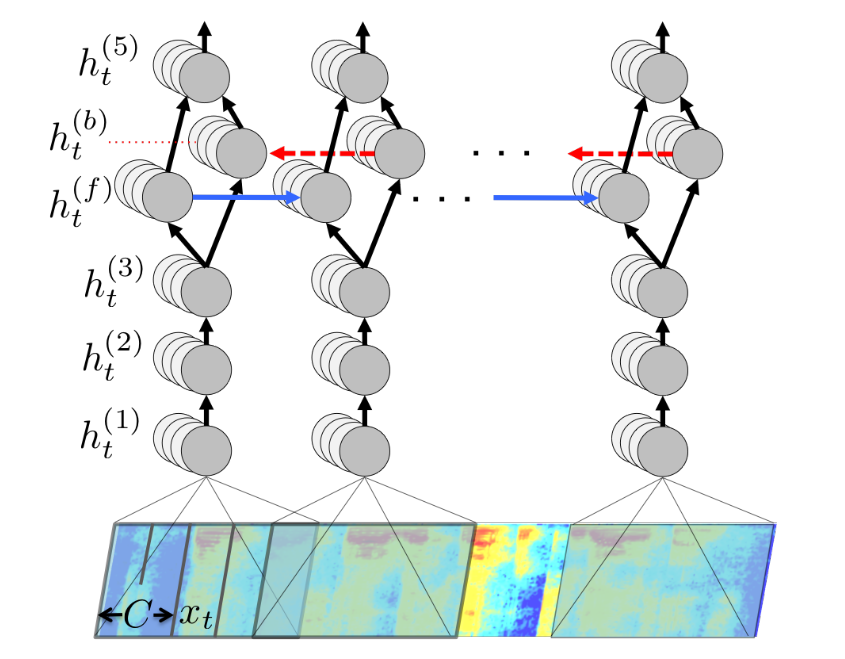
\includegraphics[width=0.5\textwidth]{images/deepspeech.png}
    \caption{Architektura modelu DeepSpeech \cite{deepspeech}}
    \label{fig:deepspeech}
\end{figure}



- efektywny CuDNN-LSTM

%Puścić model:
%- usunąć dropout
%- batch size 64 (zbyt mały batch skutkuje nistabilnym gradientem)
%- features from 5 to 10 words, increase in next epochs (koszt CTC przy dużych próbkach może powodować wybuchy gradientu, nistabilność treningu)
%Nie został on sprawdzony jak działa na języku polskim.
%
%Główne zmiany w stosunku do DS2 to m.in:
%- dwukierunkowa LSTM (lepsze wyniki) przy tym zasobie danych - nie mamy celu interakcji real
%- batch normalization cieżka do implementacji jeżeli się używa CuDNN (a inne wersje pogorszały wyniki) + nie ma tak głębokiej sieci bo nie ma tak dużo danych
%- nie ma w rnn przeskoków - nie ma takiej potrzeby (ew szybsze obliczenia / brak lepszej generalizacji)
%- LSTM zamiast GRU
%- brak data augmentation
